\documentclass[a2]{a0poster}

\usepackage[dutch]{babel}
\usepackage{url}

\pagestyle{empty}
\setcounter{secnumdepth}{0}

\usepackage[absolute]{textpos}

\usepackage{graphics}
\usepackage{wrapfig}
\usepackage{tikz}

\usepackage[T1]{fontenc} %% LGR encoding is needed for loading the package gfsneohellenic
\usepackage{arev}

\usepackage{color}
\definecolor{DarkBlue}{rgb}{0.1,0.1,0.5}

\def\SubTitle#1{\noindent{\large\color{DarkBlue} #1}\bigskip}
\def\Title#1{\noindent{\VeryHuge\color{DarkBlue} #1}}

% Set up the grid
%
% Note that [40mm,40mm] is the margin round the edge of the page --
% it is _not_ the grid size. That is always defined as
% PAGE_WIDTH/HGRID and PAGE_HEIGHT/VGRID. In this case we use
% 23 x 12. This gives us three columns of width 7 boxes, with a gap of
% width 1 in between them. 12 vertical boxes is a good number to work
% with.
%
% Note however that texblocks can be positioned fractionally as well,
% so really any convenient grid size can be used.
%
\TPGrid[40mm,40mm]{15}{12}      % 3 cols of width 7, plus 2 gaps width 1

\parindent=0pt
\parskip=0.5\baselineskip

\begin{document}

\begin{tikzpicture}[remember picture,overlay]
		\node[yshift=-0.5cm, xshift=2.5] at (current page.north west)
		{
			\begin{tikzpicture}[remember picture, overlay, rounded corners=25pt]
				\draw[line width=0.25cm, brown!30!white!90]
				(0.0,0)    -- (\paperwidth      , 0.0) -- (\paperwidth      ,-\paperheight+1.0cm) -- (0.5,-\paperheight+1.0cm) --
				(0.5,-0.5) -- (\paperwidth-0.5cm,-0.5) -- (\paperwidth-0.5cm,-\paperheight+1.5cm) -- (1.0,-\paperheight+1.5cm) --
				(1.0,-1.0) -- (\paperwidth-1.0cm,-1.0) -- (\paperwidth-1.0cm,-\paperheight+2.0cm) -- (1.5,-\paperheight+2.0cm) --
				(1.5,-1.5) -- (9.0,-1.5);
			\end{tikzpicture}

			\begin{tikzpicture}[remember picture, overlay, rounded corners=25pt]
				 \node[anchor=north west,rectangle, rounded corners=25pt,inner sep=11pt, fill=brown!30!white!90]  at (7,-1.37)
              {\Title{\fontsize{60mm}{9mm}\selectfont RFID}};
			\end{tikzpicture}

			\begin{tikzpicture}[remember picture, overlay, rounded corners=25pt]
				\node[anchor=north, rounded corners=20pt,inner sep=20pt]  at (37,-1.37)
              		{\SubTitle{\fontsize{30mm}{9mm}\selectfont in de maatschappij}};
              	\node[anchor=north, rounded corners=20pt,inner sep=11pt]  at (37,-4.37)
              		{\SubTitle{\fontsize{20mm}{19mm}\selectfont hoor en wederhoor}};
			\end{tikzpicture}

			\begin{tikzpicture}[remember picture, overlay, rounded corners=4pt]
				 \node[anchor=north west,rectangle, rounded corners=4pt, ]  at (-0.5,0.5)
              {\fontsize{4mm}{19mm}\selectfont louis onrust --- \url{l.onrust@student.science.ru.nl}};
			\end{tikzpicture}

		};
	\end{tikzpicture}


%    \begin{textblock}{wid}(x,y)
%    ...
%    \end{textblock}
%
% the first argument gives the block width in units of the grid
% cells specified above in \TPGrid; the second gives the (x,y)
% position on the grid, with the y axis pointing down.
\begin{textblock}{7}(0,1.15)
{\LARGE\color{DarkBlue} Angst, maar niet de aandacht} \small

Bij onderzoek in kranten en documentaires naar berichtgeving over RFID in de maatschappij lijkt het alsof het onderwerp niet leeft onder de
bevolking. Maar is dit wel waar? Gaan we met z'n allen akkoord met de invoering van de RFIDchip in het paspoort? Of hebben we hier met z'n
allen geen invloed op?

NRC heeft slechts 20 artikelen met de term RFID; Trouw heeft sinds 2001 slechts 63 nieuwsberichten met RFID als term gepubliceerd. Ter
vergelijking, over \emph{financi\"ele crisis} zijn meer dan duizenden berichten verschenen. Het lijkt erop alsof de lezer verzadigd is op
RFID-gebied, en er niets nieuws te melden valt.

Onderzoek van het Rathenau-instituut laat zien dat burgers onwetend zijn, en toch bang zijn voor de mogelijkheden van RFID. De media kunnen
hier op inspelen door het principe van hoor en wederhoor, maar is dit ook wat er gebeurt?
\end{textblock}

\begin{textblock}{7}(8,1.15)
{\LARGE\color{DarkBlue} Gebrek aan vertegenwoordigers} \small

De introductie van RFID-producten heeft geen herkenbare vertegenwoordiger. In krantenartikelen worden voornamelijk commerci\"ele
gebruikers, zoals boekhandels, aan het woord gelaten om de burger de voordelen van RFID in te laten zien.

Aan de andere kant is er ook geen duidelijke antagonist. Wetenschappers nemen vaak deze rol op zich of vertegenwoordigers van
privacy-organisaties.

Het gebrek aan aanspreekpunten maakt het lastig het principe van hoor en wederhoor in stand te houden. Hierdoor zijn het steeds dezelfde
mensen die hun mening verkondigen, waardoor het op den duur op een welles-nietes-strijd gaat lijken. De burger is de grote ontbrekende
speler in deze strijd. De manier om als burger mee te kunnen doen aan het debat is door zich te verenigen, zodat hoor en wederhoor weer
echt betekenis krijgt.
% Men heeft vaak een eigen visie, en
% laat zich niet zomaar be\"invloeden door een woordvoerder zonder gezag. De vertegenwoordigers die er zijn, snijden het onderwerp scherp,
% terwijl de burger bereid is concessies te maken over het gebruik van RFID in het dagelijkse leven. Burgers voelen zich hierdoor onbegrepen,
% wat funest is voor het debat.
\end{textblock}

\begin{textblock}{7}(8,6.9)
{\LARGE\color{DarkBlue} Toekomst} \small

RFID is het punt van doorbreken al voorbij, en op dit moment lijkt de opkomst niet te stoppen. De verwachting is dat
wanneer RFID een duidelijk meer zichtbare rol gaat spelen in de samenleving de debatten weer op gang komen. De vraag is dan wel of er
nieuwe argumenten aangehaald worden, of dat we weer in eenzelfde situatie komen waar er nagenoeg geen debat plaats vindt.

Mogelijkheid tot vervolgonderzoek is het onderzoeken hoe de ontvanst van RFID plaats vond in andere landen. Het is interessant om te
bekijken hoe de burger daar bij het debat betrokken is, en wat voor standpunt de burgers dan innemen. Dit vervolgonderzoek kan goed
gecombineerd worden met enqu\^etes, er kan dan gekeken worden of burgers meer aandacht willen voor RFID in de maatschappij. Of juist
bepaalde aspecten willen belichten, zoals de achterliggende techniek of de gevaren en mogelijkheden van RFID.
\end{textblock}

\begin{textblock}{7}(0,6.9)
{\LARGE\color{DarkBlue} Resultaten} \small

De meeste berichten zijn eenzijdig: ze zijn ofwel positief over RFID of ze voorspellen onheil door RFID. Van de onderzochte krantenberichten
begonnen alswel eindigden \(44\%\) met een negatief beeld, en \(22\%\) van de nieuwsberichten begonnen en eindigden onbesloten. Dit duidt
erop dat de berichtgeving in balans is. Toch brengt \(77\%\) van de berichten RFID in verband met schending van privacy.

De mening van de burger wordt meegedeeld door de journalist, er komt in de artikelen nooit een burger aan het woord. Hierdoor kan de
burger zichzelf nooit rechtstreeks verdedigen en wordt een van de belangrijkste participanten aan het debat uitgesloten. De ``onwetendheid''
van de burger is herleidbaar tot het onbeslisbaar zijn en het krijgen van vage en inaccurate berichtgeving.

De resultaten laten zien dat het laatste woord nog niet gezegd is over RFID: dit weerspiegelt goed het huidige maatschappelijke klimaat.
\end{textblock}

\end{document}